%André Fernandes dos Santos
%LEI, nº49344

\documentclass{article}
\usepackage[portuguese,english]{babel}
\usepackage[utf8]{inputenc}
\usepackage[T1]{fontenc}
\usepackage{a4wide}
\usepackage{txfonts}% use Arial && Times New Roman
\usepackage[pdftex]{color,graphicx}
\usepackage{fancyhdr}
\usepackage{fancyvrb}
\usepackage{cite}
\usepackage{longtable}
\usepackage{verbatim}
\usepackage{ae}
\usepackage{multicol}
\usepackage{graphicx}
\usepackage{hyperref}
\usepackage{url}

\renewcommand\familydefault{\sfdefault}% usar font sem serifas
\renewcommand{\labelitemi}{$-$}
\author{André Fernandes dos Santos}
\title{Curriculum Vit\ae}
\date{\today}

\begin{document}
\maketitle
\thispagestyle{empty}

\newpage
\section{Personal Information}
	\begin{description}
	%\item [Nome:] \framebox{\textsc{André Fernandes dos Santos}}
	\item [Name:] \textbf{\textsc{André Fernandes dos Santos}}
	\item [Birthdate:] 24 February 1988
	\item [Address:] Pq. Resid. Fonte Seca, Lt8B 1$\,^{\circ}$E, 4715-229 BRAGA
	\item [Civil state:] Single
	\item [Mobile number:] +351 92 77 15 379
	\item [Email:] pg15973@alunos.uminho.pt
	\end{description}

%	\begin{figure}[htbp]
%	\centering
%	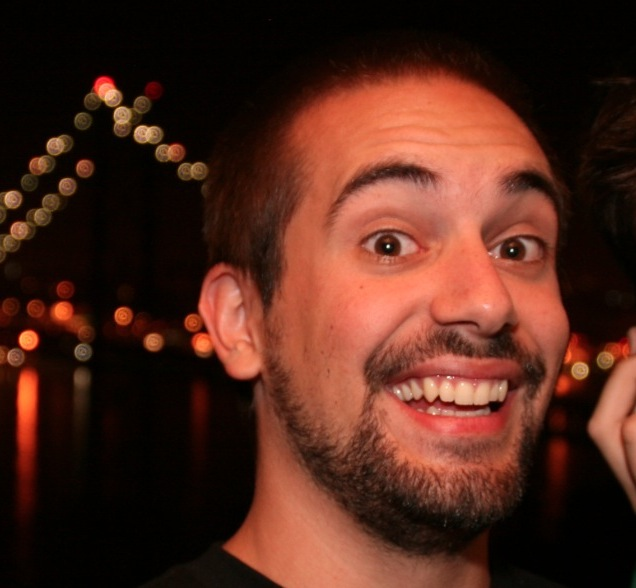
\includegraphics[width=.1\textwidth]{foto}
%	\end{figure}

	\vspace{.2cm}
	\begin{description}
		\item [Twitter:] \texttt{@about\_andrefs} 
		\item [GitHub:] \url{github.com/andrefs} 
		\item [LinkedIn:] \url{linkedin.com/in/andrefs}
		\item [SlideShare:] \url{slideshare.net/andrefsantos}
	\end{description}


\section{Education}
\begin{description}
\item [2006-2009] Degree in Software Engineering, University of Minho (180 ECTS, final grade 14.56/20.00)
\item [2009/2010] 1${^\textrm{st}}$ year of Software Engineering MSc, University of Minho (120 ECTS)
	\begin{itemize}
		\item Languages Engineering (final grade 16/20)
		\item Bioinformatics (final grade 16/20)
	\end{itemize}
\item [2010/2011] Advanced Bioinformatics and Systems Biology (extracurricular subject, 30 ECTS)
\item [2010/present] 2${^\textrm{nd}}$ year of Software Engineering MSc, University of Minho
	\begin{itemize}
		\item Master thesis: ``Building a Corpora-Flow System''\\
		Development of a system to support automatic handling of corpora (cleaning, validation, format conversion), document alignment and estimate the alignability of several types of documents, as well as make them available on the internet.
	\end{itemize}
\end{description}

\section {Training}
\begin {description}
\item [Jul 2005] German Open Course, U. Junior, Faculty of Arts, University of Porto
\item [Set 2005] Physics Summer School, Faculty of Science, University of Porto
\item [Jun 2010] Catalyst 5.80 (\textit{Portuguese Perl Workshop 2010}, Porto)
\item [Jul 2010] Evolutionary Computing School, (UMinho, Guimarães)
\item [Out 2010] Seminar ``Republic and Youth'', National Youth Council
\item [Nov 2010 - Mar 2011] IdeaLab -- Business Ideas Lab, TecMinho
\item [Jun 2011 - Jul 2011] Summer School on Conceptual Design and Development of Innovative Products 2011, Struer, Denmark (5 ECTS)
\end{description}

\section{Professional Experience}
\begin{description}
\item [Jul-Set 2009] Project Bigorna, Traineeship Sapo Summerbits 2009\\
\url{http://natura.di.uminho.pt/wiki/doku.php?id=ferramentas:bigorna}\\
Open source project which aims to develop tools to help in general orthography migration challenges, motivated by the 1990 Portuguese Language Orthographic Agreement.
\item [Feb 2011 - present] Systems Administrator at GroupBuddies\\
\url{http://www.groupbuddies.com}\\
Startup company which develops web-based solutions for groups and organizations. Typical tasks include:
\begin{itemize}
	\item deployment and management of several Unix-based servers
	\item managing Ruby on Rails applications on a production environment
	\item managing Git repositories
	\item development of helper scripts to automate and facilitate server management
	\end{itemize}
\item [Apr 2011 - present] Scholarship from project \textit{Per-Fide: Portuguese in parallel with six languages: Español, Russian, Français, Italiano, Deutsch, English}.\\
Project devoted to build a large parallel corpora.

\end{description}

\section{Technical Skills}
\begin{description}
\item[-] Basic experience with PASCAL, C\#, PHP, JavaScript, UML, XML, Html, SQL, Haskell;
\item[-] Experience with C and Java;
\item[-] Proficiency with  Perl, including Moose, Catalyst, Dancer, DBIx::Class and other Modern::Perl concepts;
\item[-] Unix sys admin experience;
\item[-] Others: \LaTeX, bash, Subversion, Git, Apache and associated technologies.
\end{description}

\section{Other Activities}

\subsection{CeSIUM (UMinho's Software Engineering Student Center)}
\begin{description}
	\item [2008-2011] Member of CeSIUM 
	\item [2009/2010] Vice-President of CeSIUM 
	\item [2010/2011] Director of CAOS (Open Source Support Center)
\end{description}
\subsection{Programming Challenges}
\begin{description}
	\item [Out 2007] Inter-University Programming Marathon (IST, UTL, Lisbon)
	\item [Out 2008] Inter-University Programming Marathon (UC, Coimbra)
	\item [Nov 2008] ACM South Western European Regional Contests (Nuremberg, Germany)
	\item [Out 2009] Inter-University Programming Marathon (ESTGA, Aveiro)
\end{description}
\subsection{Sports}
\begin{description}
	\item [1998-2000] Artistic gymnastics
	\item [2007-2008] Basketball
	\item [1999-2011] Judo, 4$\,^{\textrm{th}}$~Kyu
	\item [Mar 2010] National Judo University Championship, Aveiro
	\item [Mar 2011] National Judo University Championship, Lisbon
\end{description}

\renewcommand{\refname}{\section{Publications}}
\bibliographystyle{plain}
\bibliography{aspubs}
\nocite{*}

\end{document}

